\section{Simulation preparation}
Now that we have the equations that govern the motion of a satellite in place we can proceed to write a computer program that will simulate the trajectory a satellite takes after it is put in orbit. When a satellite is placed in its orbit it will have values of \(r\) and \(\nu\) change as time goes by. This coupled with inclination of the orbit will aid in locating the position of the satellite in its orbit.

The diagram below illustrates the elements used to locate a satellite in its orbit;
\begin{figure}[h]
	\centering
	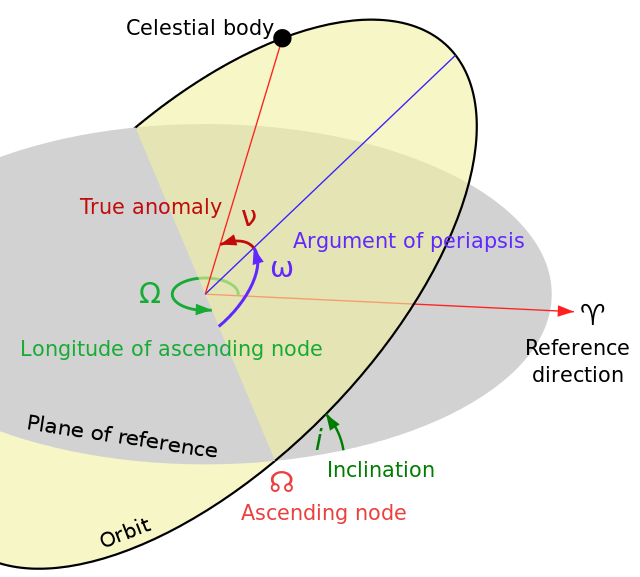
\includegraphics[width=0.4\textwidth]{orbit}
	\caption{Orbital elements for a satellite.}
	\label{fig:six-orbital-elements}
\end{figure}

\subsection{Satellite launch data acquisition}
For each satellite launched into space the data of it's launch variables are provided by NASA and can be acquired from \textcite{http://celestrak.com}. Of particular interest is the Kenyan satellite launched into space in the year 2018. The particular launch data is at \textcite{http://celestrak.com/satcat/tle.php?CATNR=43467}. This will give us a two-line-element from which we will extract the particular values for the satellite of interest.

From the Two-Line-Element we will be able to deduce the orbital elements of 1KUNS-PF namely its eccentricity, mean anomaly, mean motion and the Argument of Perigee.


The Two-Line-Element for 1KUNS-PF is this;\\
\textcite{1KUNS-PF}\\              
\textcite{1 43467U 98067NQ  18290.48306199  .00009882  00000-0  13782-3 0  9995}\\
\textcite{2 43467  51.6385 126.6004 0002599 213.4711 146.6117 15.57589009 24750}\\

From this we are able to define inclination=51.6385, eccentricity=0.002599, mean anomaly=146.6117, mean motion=15.57589009 and the Argument of Perigee=213.4711.

We will use this values to write a computer program that will simulate the trajectory that 1KUNS-PF will follow.

We also use celestrak to acquire more data for cubesats that were launched in 2018. This data will be used to simulate multiple satellites orbiting the earth.

\subsection{Position Simulation Algorithmn}
The algorithmn we will use to determine the position of the satellite;\\
\begin{description}
	\item[1.] Set the values that define the satellite orbit.
	\item[2.] Set the time to the required start position and set the time step for simulation.
	\item[3.] Get the initial values for the orbital elements for the satellite.
	\item[4.] Convert these values from polar coordinates to cartesian coordinates.
	\item[5.] Plot the cartesian values in a 3 dimensional graph.
	\item[6.] Plot the orbit for the satellite.
	\item[7.] Plot the earth in 3 dimensions using the standard lengths.
	\item[8.] Increment the time step.
	\item[9.] Repeat step 1-8 with updated values for the satellite position.
\end{description}

The code that implements this algorithmn has been further discussed in the appendix in much detail. The language of choice used in this simulation is Python as it is rich with scientific tools, has a good community and fully-fledged libraries. Matplotlib, numpy and jupyter notebook were employed in the creation of these simulations.

Numpy has been used to work the numbers into a suitable format to work with. Matplotlib has been used for the plotting and simulation itself. Jupyter was used for development purposes.
\subsection{Time step}
For this particular case we will use the default timestep provided by matplotlib FuncAnimation library. This will ensure that we only get to worry about the position itself and not how the display of the animation works.
\\
\\
\\
\section{Simulation}
\subsection{Dummy satellite simulation}
The simulation was done for a dummy satellite as shown below;
\begin{figure}[h]
	\centering
	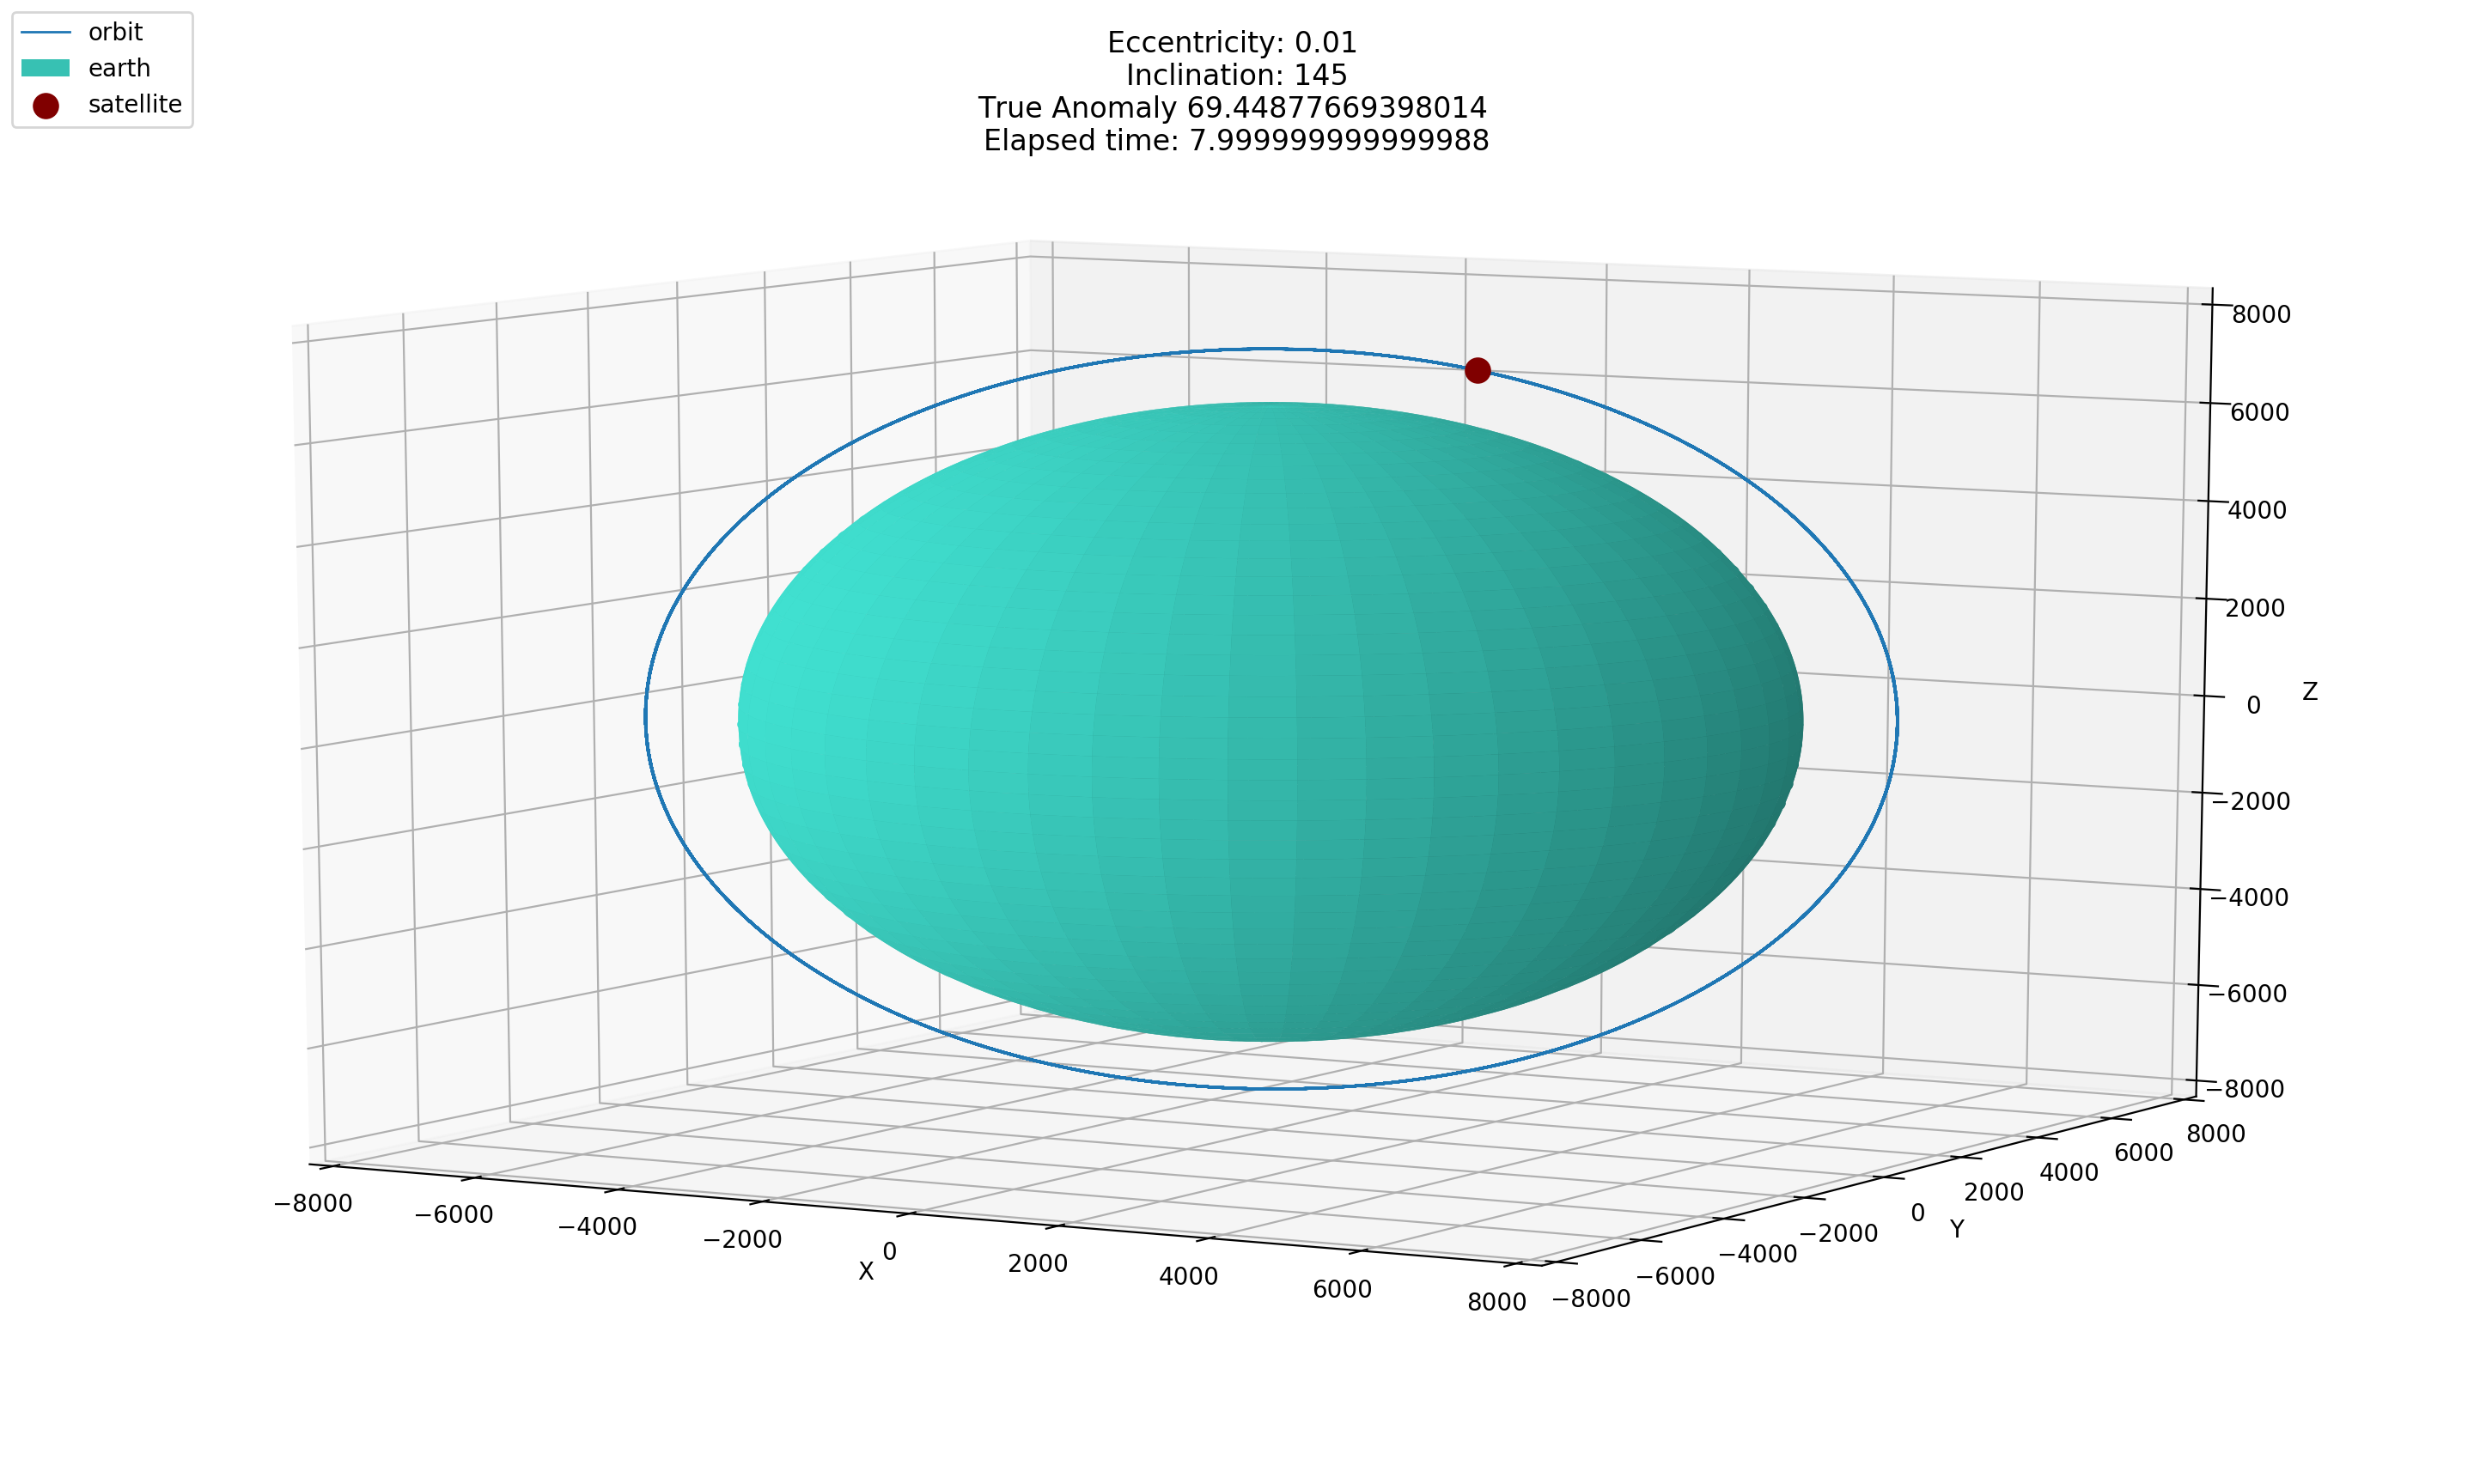
\includegraphics[width=1.2\textwidth]{3d_satellite}
	\caption{Dummy satellite: elev=10., azim=-60.}
	\label{fig:dummy-satellite}
\end{figure}

The values used for this satellite were; dummy-sat = Satellite(1, 0.01, 7500, 145, 69)   where Satellite(mass, eccentricity, semi-major-axis, inclination, true-anomaly) is the python class that defines the satellite.

The satellite is moving in a medium earth orbit \textbf{LEO} with a retrogade motion\big(moving in a different direction as the rotation of the earth). The altitude of the satellite of the satellite at perigee is 1046.85km.

\subsection{1KUNS-PF satellite simulation}
The simulation was done for 1KUNS-PF satellite, with semi-major axis being 6778.8km, as shown below in Figure 4.3.
\begin{figure}[h]
	\centering
	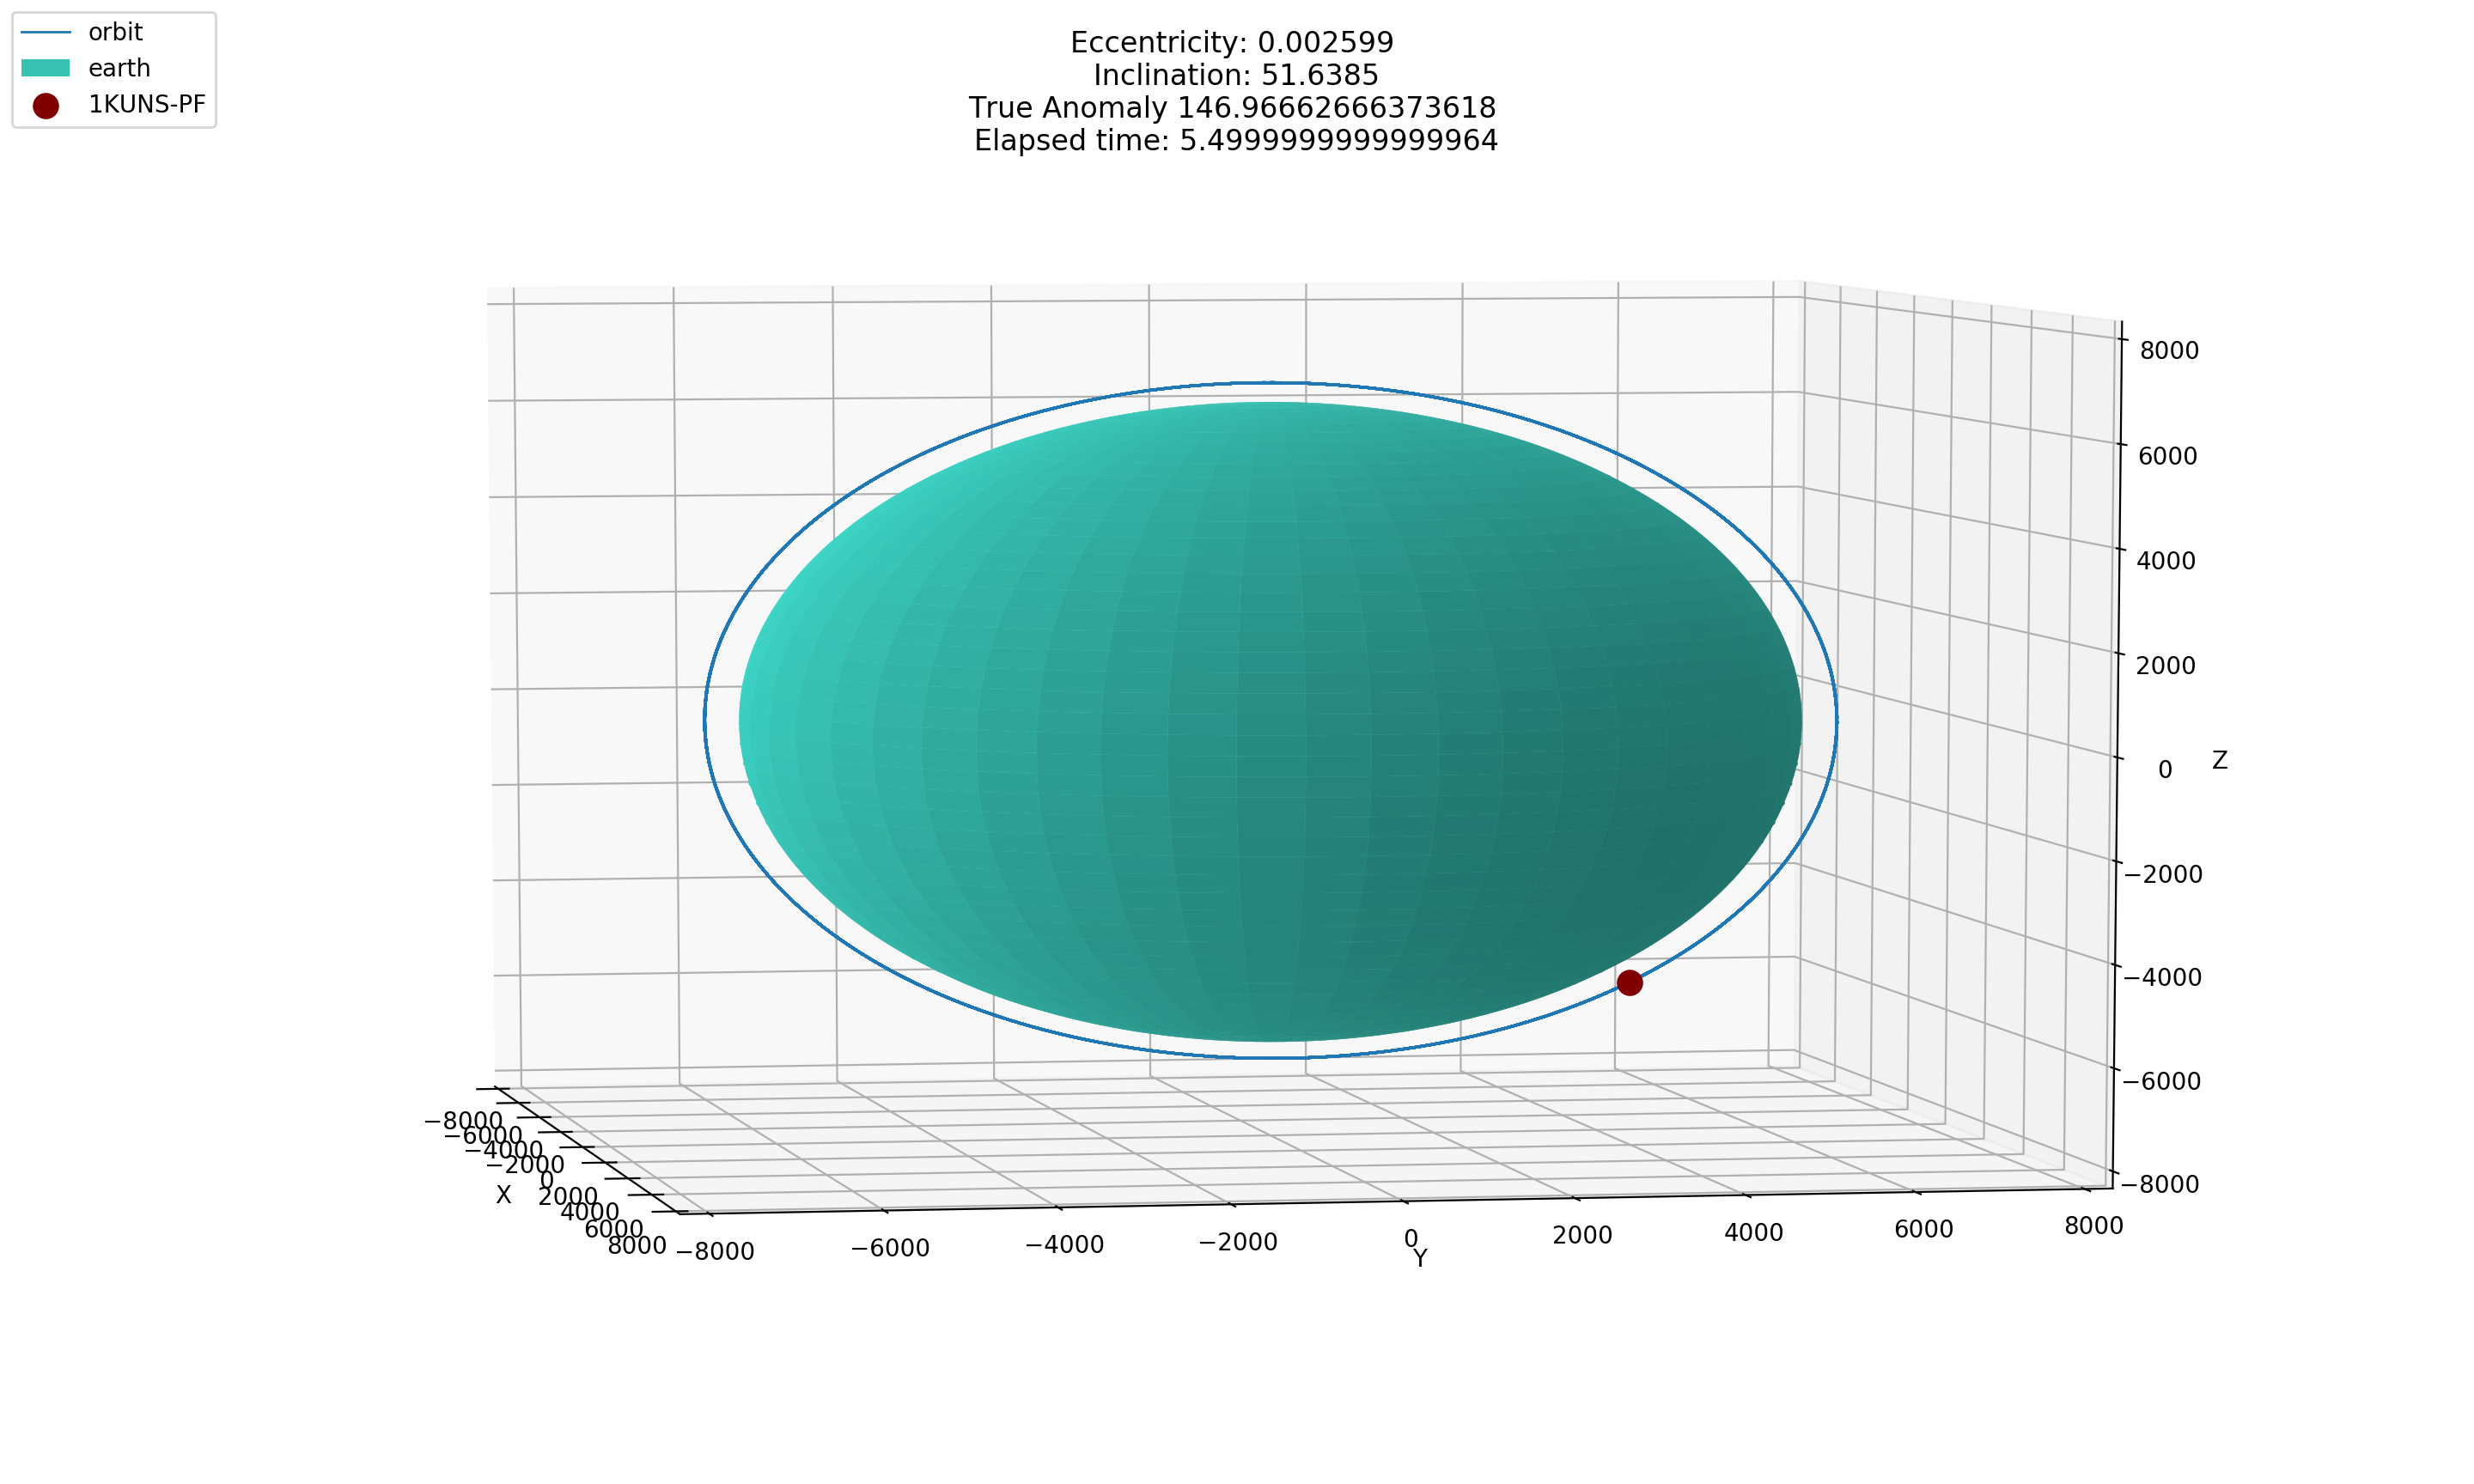
\includegraphics[width=1.2\textwidth]{1kuns-pf}
	\caption{1KUNS-PF: elev=-10., azim=5.}
	\label{fig:1KUNS-PF}
\end{figure}

The values used for this satellite were; kuns = Satellite(1, 0.002599, 6778.8, 51.6385, 146.6117)   where Satellite(mass, eccentricity, semi-major-axis, inclination, true-anomaly) is the python class that defines the satellite.

The satellite is moving in a low earth orbit \textbf{LEO} with a posgrade motion, moving in the same direction as the rotation of the earth. The altitude of the satellite of the satellite at perigee is 383.04km. This is quite close as compared with the actual figure which 398.9 km according to 
\textbf{https://www.n2yo.com/satellite/?s=43466}.
\subsection{3-Body simulation: 1KUNS-PF and Dummy-Sat satellite simulation}
The simulation was done for 1KUNS-PF satellite and the dummy sat as shown in Figure 4.4. The values used for this satellite were; kuns = Satellite(1, 0.002599, 6778.8, 51.6385, 146.6117)  and dummy-sat = Satellite(1, 0.01, 7500, 145, 69) where Satellite(mass, eccentricity, semi-major-axis, inclination, true-anomaly) is the python class that defines the satellite.

For this case we have use matplolib's plot-wireframe method to represent the earth in 3-d dimensions.

In this case we define \(r_{kuns}\) and \(r_{dummy}\) for 1KUNS-PF and dummy-sat respectively as;
\[r_{kuns}=\frac{a_{kuns}\big(1-e_{kuns}^2)}{1+e_{kuns} \cos \nu_{kuns}} \]
\[r_{dummy}=\frac{a_{dummy}\big(1-e_{dummy}^2)}{1+e_{dummy} \cos \nu_{dummy}} \]

This will give a wireframe figure as an attempt towards simulation of the three body-problem.
\begin{figure}[h]
	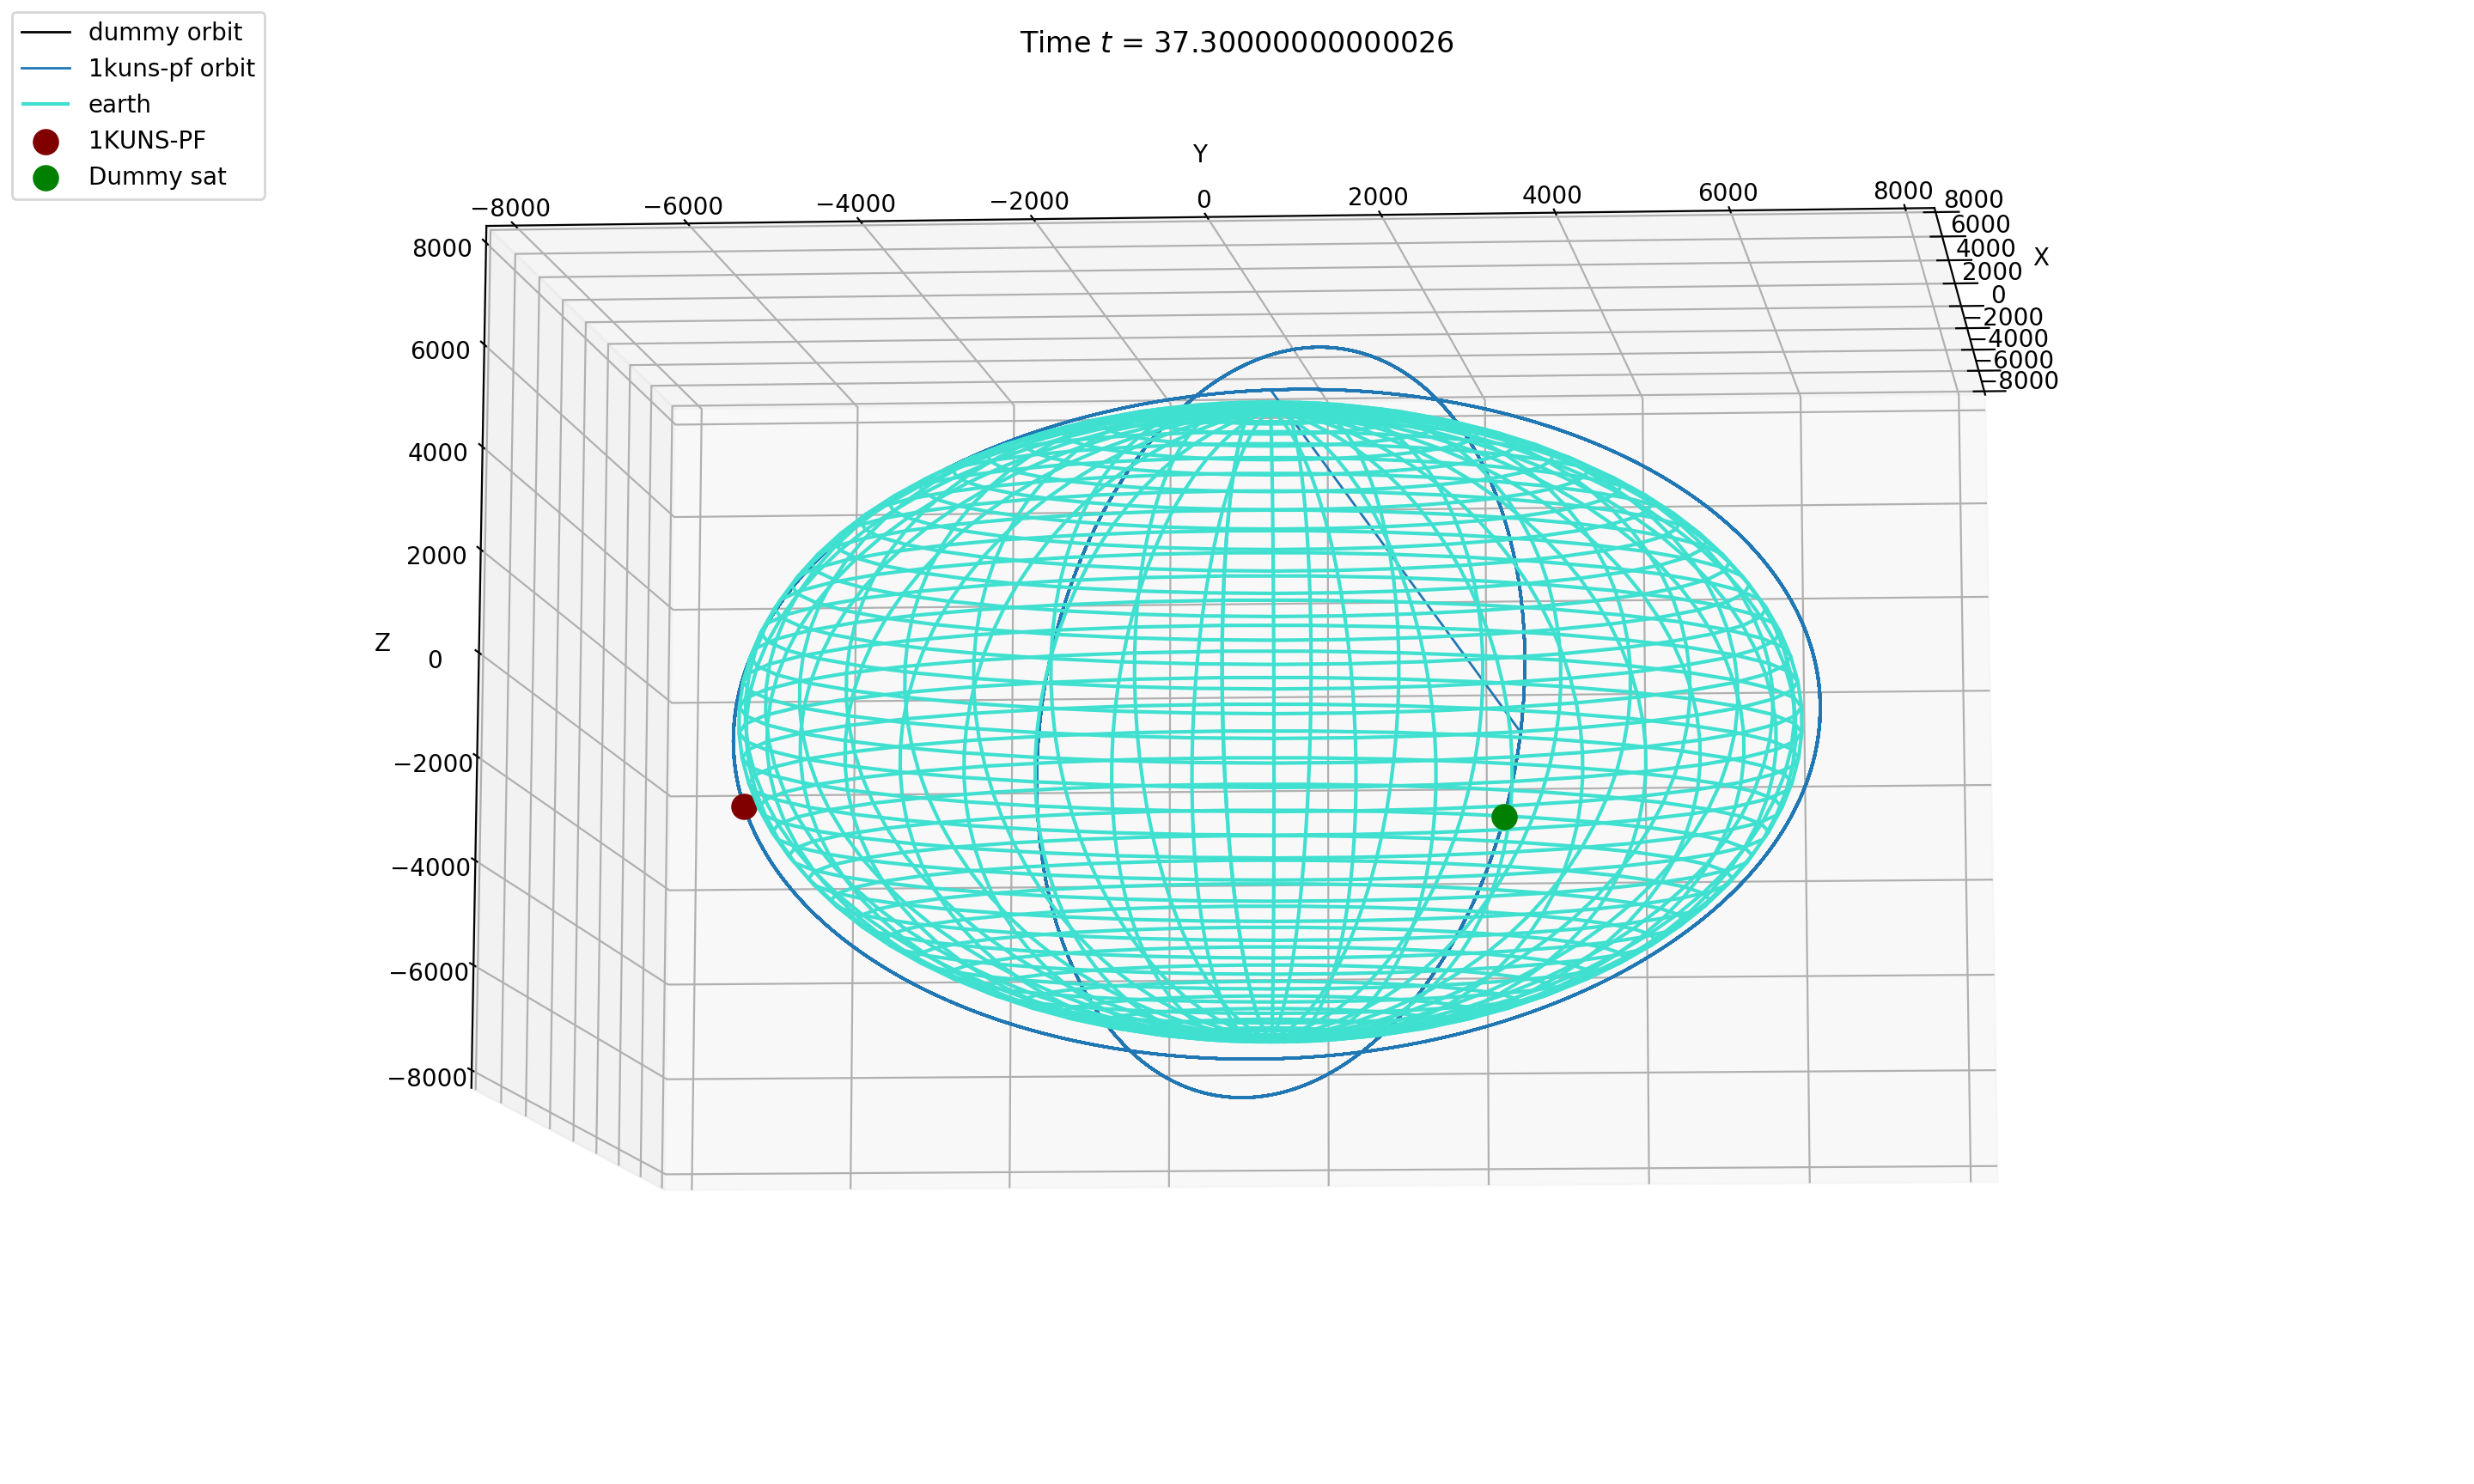
\includegraphics[width=1.2\textwidth]{3body}
	\caption{3-body simulation: 1KUNS-PF and Dummy-sat elev=-10., azim=5.}
	\label{fig:3body-sim}
\end{figure}	




